%%%%%%%%%%%%%%%%%%%%%%%%%%%%%%%%%%%%%%%%%
% Twenty Seconds Resume/CV
% LaTeX Template
% Version 1.1 (8/1/17)
%
% This template has been downloaded from:
% http://www.LaTeXTemplates.com
%
% Original author:
% Carmine Spagnuolo (cspagnuolo@unisa.it) with major modifications by 
% Vel (vel@LaTeXTemplates.com)
%
% License:
% The MIT License (see included LICENSE file)
%
%%%%%%%%%%%%%%%%%%%%%%%%%%%%%%%%%%%%%%%%%

%----------------------------------------------------------------------------------------
%	PACKAGES AND OTHER DOCUMENT CONFIGURATIONS
%----------------------------------------------------------------------------------------

\documentclass[letterpaper]{twentysecondcv} % a4paper for A4

\usepackage[super]{nth}
\usepackage{enumitem}

\setitemize{noitemsep,topsep=0pt,parsep=0pt,partopsep=0pt}

%----------------------------------------------------------------------------------------
%	 PERSONAL INFORMATION
%----------------------------------------------------------------------------------------

\profilepic{}

\cvname{Mostafa Abdelaziz}
\cvjobtitle{Computer and Systems Engineer}

\cvdate{} % it is preferred not to put your age in Canada
\cvaddress{\vspace{-12px}
           111 Bannatyne Dr.\newline
           Toronto, ON \hspace{4px} M2L 2P5}
\cvnumberphone{+1 778-788-0657}
\cvmail{\href{mailto://iocoder@aol.com}{iocoder@aol.com}}
\cvsite{\href{https://iocoder.github.io/}{https://iocoder.github.io}}
\cvlinkedin{\href{http://www.linkedin.com/in/mabdelaz/}{linkedin.com/in/mabdelaz}}

%----------------------------------------------------------------------------------------

\begin{document}

%----------------------------------------------------------------------------------------
%	 ABOUT ME
%----------------------------------------------------------------------------------------

\aboutme{Computer software engineer with wide technical expertise in software engineering,
         computer networks, database systems, computer architecture, and embedded
         systems.}

%----------------------------------------------------------------------------------------
%	 SKILLS
%----------------------------------------------------------------------------------------

\skills{
    \center{
        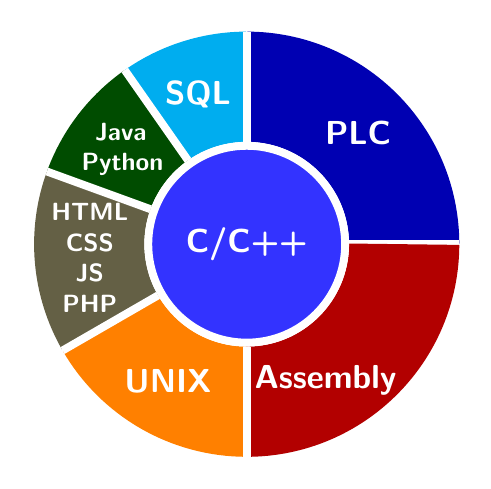
\begin{tikzpicture}[font=\sffamily\bfseries\large, text=white, border/.style={line width=14mm}]
        \foreach \angle/\col [remember=\angle as \last (initially 0)] in 
            {90/blue!70!black, 125/cyan, 160/green!30!black, 210/yellow!30!black, 270/orange, 360/red!70!black}{
                \draw[\col, border] (\last:2cm) 
                     arc[start angle=\last, end angle=\angle, radius=2cm];
                \draw[white, line width=1mm] (\last:1.3)--++(\last:1.4);
        }
        \node[line width=1mm, draw, circle, minimum width=2.5cm, white, fill=blue!80] {C/C++};
        \node at (45:2cm) {PLC};
        \node at (108:2cm) {SQL};
        \node[text width=1cm, align=center, font=\sffamily\bfseries\small] at (143:2cm) 
            {Java Python};
        \node[text width=1cm, align=center, font=\sffamily\bfseries\small] at (185:2cm) 
            {HTML CSS JS PHP};
        \node at (240:2cm) {UNIX};
        \node at (300:2cm) {Assembly};
        \end{tikzpicture}
    }
}

%----------------------------------------------------------------------------------------
%	 OS PREFERENCES
%----------------------------------------------------------------------------------------

\ospref{
    \textcolor{black}{
    \textbf{GNU/Linux}\hfill
\includegraphics[scale=0.40]{../img/5stars.png}\newline
    \textbf{FreeBSD}\hfill
\includegraphics[scale=0.40]{../img/4stars.png}\newline
    \textbf{Windows}\hfill
\includegraphics[scale=0.40]{../img/4stars.png}}}

%----------------------------------------------------------------------------------------
%	 LANGUAGES
%----------------------------------------------------------------------------------------

\langs{{Italian (\textit{Beginner})/2},{Arabic (\textit{Native})/6},{English (\textit{IELTS 7.5})/5}}

%----------------------------------------------------------------------------------------
%	 COURSES
%----------------------------------------------------------------------------------------

\courses{
    Academic Course Highlights: Programming, OOP, Software Engineering,
    Data Mining, AI, Data Structures, File Organization, Databases,
    Algorithm Analysis, OS, Compilers, Computer Architecture, Embedded
    Systems, and Networks.
}

%----------------------------------------------------------------------------------------

% Print the sidebar
\makeprofile

%----------------------------------------------------------------------------------------
%	 EDUCATION
%----------------------------------------------------------------------------------------

\section{Education}

\begin{twenty} % Environment for a list with descriptions
	%\twentyitem{<dates>}{<title>}{<location>}{<description>}
	\twentyitem{2011 - 2016}
               {B.Sc., Computer and Systems Engineering}
               {Alexandria University}
               {\textbf{GPA}: 3.94.\newline
                \textbf{Overall Ranking}: \underline{\nth{1}}.\newline
                \textbf{Graduation Project}: FPGA computer based on MIPS architecture.\newline
                \textbf{WES Evaluation}: currently in progress.\newline
                %\textbf{Course Highlights}: Control Theory, Modern Control, Embedded Systems,
                %                            Computer Architecture, Software Engineering,
                %                            System Software, Operating Systems, Compilers, Switching Theory,
                %                            Automata Theory, Complexity Theory.
               }
	\twentyitem{2008 - 2011}
               {High School}
               {Mubarak Secondary School, Alexandria}
               {\textbf{Overall Grade}: 407.5/410 (99.36\%).\newline
                \textbf{Specialization}: Mathematics.}
\end{twenty}

%----------------------------------------------------------------------------------------
%	 EXPERIENCE
%----------------------------------------------------------------------------------------

\section{Experience}

\begin{twenty}
	\twentyitem{\hspace{2ex} 2017}
               {Research Assistant}
               {Simon Fraser University, BC}
               {Implementation of an LTE base station using \textit{Ettus B210 USRP} and \textit{OpenAirInterface}.
               }

	\twentyitem{\hspace{2ex} 2017}
               {Control Systems Engineer}
               {Advanced HVAC Consultant, Cairo}
               {Implementation of feedback control loops for HVAC systems using \textit{Fupla} (function block diagrams) on 
                \textit{Saia Burgess PLC} devices. The work included:
                \begin{enumerate}
                    \item{Control loops for airhand units (fans, valves, and sensors).}
                    \item{Control loops for chillers and water pumps.}
                    \item{Interfacing \textit{Saia Burgess PLCs} and \textit{Honeywell Eagle DDCs} using 
                          Modbus and Bacnet/IP.}
                    \item{Developing interactive Human-Computer Interfaces using \textit{Tridium controller}
                          to interface the human operator with PLC logic.}
                    \item{Instructing our teams on the implementation of electrical boards composed of
                          high-voltage relays and networks of PLCs and RIOs.}
                    \item{Troubleshooting and solving technical problems at the field.}
                \end{enumerate}
               }

	\twentyitem{\hspace{2ex} 2016}
               {Software Engineer}
               {Ejada Systems Ltd., Alexandria}
               {Providing enterprise solutions to banks in the Middle East, including:
                \begin{enumerate}
                    \item Implementation of \textbf{CRM} systems using \textbf{Oracle Siebel}.
                    \item Developing \textbf{BigData} solutions using
                          \textbf{Hadoop} and \textbf{Scala}.
                \end{enumerate}}

	\twentyitem{\hspace{2ex} 2015}
               {RA Intern}
               {SmartCI Research Center, Alexandria}
               {Programming the storage system of a cognitive radio cloud, which consisted of
                Linux nodes with ext2fs, using IP multicast and filesystem-aware data compression.}

	%\twentyitem{<dates>}{<title>}{<location>}{<description>}
\end{twenty}

%----------------------------------------------------------------------------------------
%	 PUBLICATIONS
%----------------------------------------------------------------------------------------

\section{Selected Projects}

\begin{itemize}
    \item{Quafios: An Operating System for x86 and MIPS. The system included:
          \begin{itemize}
            \item Implementation of a UNIX-like system call interface.
            \item Device drivers for PCI, USB, ATA, timers, interrupt controller, 
                  keyboard controller, and other hardware components.
            \item Dynamic kernel-space and user-space memory allocation algorithms.
            \item Implementation for C library routines.
            \item A GUI, with a programmer-friendly API.
          \end{itemize}
          }
    \item{Compilter for subset of C and Java Programming Languages}
    %\item{Systema Programming Language and Compiler.}
    %\item{Radio KAOS: Cognitive Radio with Dynamic Spectrum Sharing Engine.}
    \item{CDP: Reliable Data Transfer Protocol for Linux Kernel TCP/IP Stack.}
    \item{Designed a Linux kernel device driver and synchronization assignment 
          for OS course at Alexandria University.}
    \item{Liftroid: Visualized elevator Android interface with AVR.}
    \item{Technical Report on \textit{Unified Extensible Firmware Interface}.}
    %\item{IDE to USB interface using AVR and PIC.}
    %\item{8086 micro-computer system.}
    %\item{System for OS image distribution over cloud using Frisbee.}
    %\item{QCC C/Java Compiler for GNU/Linux.}
    %\item{NES (Nintendo Entertainment System) Simulator.}
    %\item{Hello World BIOS.}
    %\item{Static RAM with MOSFETs on PCB.}
    %\item{T-DEC/102, a simulated TTL computer.}
    %\item{Educational Program with Animated Agent for Disabled Children.}
\end{itemize}

%----------------------------------------------------------------------------------------
%	 AWARDS
%----------------------------------------------------------------------------------------

\section{Selected Awards}

\begin{twentyshort}
	\twentyitemshort{2017}       {CSED Golden Armor for the \textbf{Top Student} of 2015-2016 Class.}
	\twentyitemshort{2017}       {Prof. Naeem Abou Taleb Award for \textbf{Top Student}.}
	\twentyitemshort{2012 - 2016}{\textbf{Certificate of Excellence}, Alexandria University.}
	%\twentyitemshort{<dates>}{<title/description>}
\end{twentyshort}

\vfill
\footnotesize{
\begin{itemize}[leftmargin=10px]
    \item[--] You can find the \LaTeX source code of my resume at \color{blue}{
                 \href{http://www.github.com/iocoder/resume}{http://www.github.com/iocoder/resume}}.
\end{itemize}
}

\end{document} 
